\chapter{Our Contribution : A Learning-Informed Masking Framework for Multi-Agent Representation Learning}


% \section*{Introduction : From General Inference to Policy-Relevant Representation}

% In this chapter, we present the findings from our experiments and provide an analysis of the results. We will explore the performance of the baseline algorithms and the impact of various modifications and enhancements on these algorithms. The chapter is structured to discuss the results obtained from different experimental setups, analyze the implications of these results, and interpret their significance in the context of our research objectives. Our primary focus is on understanding how the introduced methods affect the stability, convergence, and overall effectiveness of the techniques we presented in Chapter 3 in our given MARL environment.

% The previous chapter established the Multi-Agent Masked Auto-Encoder (${MA}^2E$) as a powerful method for inferring global information from local observations \parencite{ma2e}. While its self-supervised objective is effective, a critical analysis of its training methodology reveals a key limitation: the use of a policy-agnostic, random masking strategy during the fine-tuning phase.

% This chapter argues that for optimal performance, the self-supervised reconstruction task must be dynamically aligned with the agents' evolving policies. We introduce a novel framework that scores agent performance in real-time and uses this information to intelligently mask the most uncertain or \textit{poorly learning} agents. This forces the ${MA}^2E$'s representational power to focus where it is needed most, creating a more efficient and effective learning curriculum.
\section*{Introduction }
The previous chapter established the Multi-Agent Masked Auto-Encoder (${MA}^2E$ ) \parencite{ma2e} as a powerful method for inferring global information from local observations. The central thesis of our work is that to create the most effective environmental representations, the inference process itself should be guided by information from the agents' own training dynamics.

A critical analysis of the original ${MA}^2E$  methodology reveals a key limitation in this regard: use of a policy-independent and randomly applied masking strategy during  training masked auto encoder . This random approach creates a disconnect between the self-supervised reconstruction task and the primary reinforcement learning objective.

This chapter argues that for optimal performance, these two tasks must be dynamically aligned. We introduce a novel framework that scores agent performance in real-time and uses this information to intelligently mask the most uncertain or \textit{poorly learning} agents. This forces the ${MA}^2E$ 's representational power to focus where it is needed most, creating a more efficient and effective learning curriculum.
% \subsection{Preliminaries: The Masked Auto-Encoder}

\section{The Masked Auto-Encoder}
\label{section:mae_original}
% At the core of our approach is the Masked Auto-Encoder (MAE), a powerful self-supervised learning model that has demonstrated remarkable success in representation learning, particularly in computer vision \parencite{maskedautoencoder}. An MAE learns robust latent representations by solving a challenging self-supervised task: reconstructing a complete input signal from a heavily corrupted, partial version.
\begin{figure}[H] 
    \centering
    % Box for the image
        % \includegraphics[width=\linewidth]
         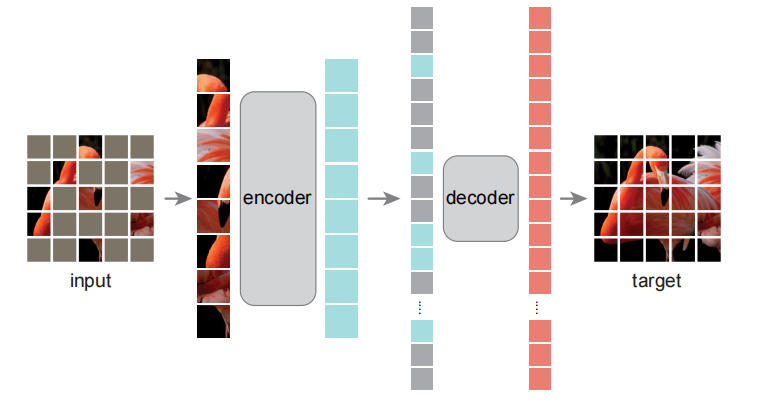
\includegraphics[width=0.8\linewidth]{img_pfe/mae_original.PNG}
   
    
        \caption{MAE architecture. (Adapted from \parencite{maskedautoencoder}).}
        \label{fig:mae_original}
\end{figure}
% \subsection{Preliminaries: A Detailed Examination of the Masked Auto-Encoder}
At the core of our approach is the Masked Auto-Encoder (${MAE}$ )  \parencite{maskedautoencoder}, a self-supervised learning paradigm that represents a significant shift in representation learning. Unlike contrastive methods that learn by comparing different views of data, MAE learns by solving a generative, reconstruction-based task. The core philosophy is to corrupt a signal and train a model to restore it, compelling the model to internalize the data's underlying structure and semantics. This section provides a detailed, step-by-step deconstruction of the ${MAE}$  framework.

% \subsubsection*{The MAE Pipeline: From Corrupted Input to Semantic Representation}
\subsection*{The ${MA}E$  Pipeline :[Figure \ref{fig:mae_original}]}
% The MAE process can be understood as a sequence of carefully designed steps, each with a specific purpose that contributes to the model's overall effectiveness and efficiency.

\paragraph{Input tokenization} The process begins with input tokenization, where the image is deconstructed into a sequence of discrete elements. The image is divided into a regular grid of non-overlapping patches (e.g., 16x16 pixels), each flattened into a vector and linearly projected to a fixed dimension, creating \textit{visual tokens}. A linear embedding layer performs this transformation, with learnable positional embeddings added to retain spatial information. This step is crucial as it converts the image into a sequence format compatible with Transformer architectures while avoiding redundancy from overlapping regions.
% \paragraph{Aggressive random masking}
\paragraph{Random masking} Next, aggressive random masking is applied, where a large, random subset of tokens (often 75\% or more) is discarded. This high masking ratio is essential to  prevents the model from relying on low-level spatial redundancy and instead forces it to develop a high-level understanding of the image to reconstruct missing parts effectively. The masking is performed via uniform random sampling, leaving only a small fraction of tokens visible.

\paragraph{Asymmetric encoder} The asymmetric encoder, a Vision Transformer (ViT) \parencite{vit}, processes only the unmasked tokens. 
% This design choice is key to MAE's efficiency: since the encoder operates on just 25\% of the data (for a 75\% masking ratio), it dramatically reduces computational cost while still learning rich semantic representations. 
The encoder employs multi-head self-attention to model relationships between tokens, building context-aware features, as illustrated in Figure \ref{fig:vit}.
% \paragraph{Lightweight decoder}
\begin{figure}[H]
    \centering
    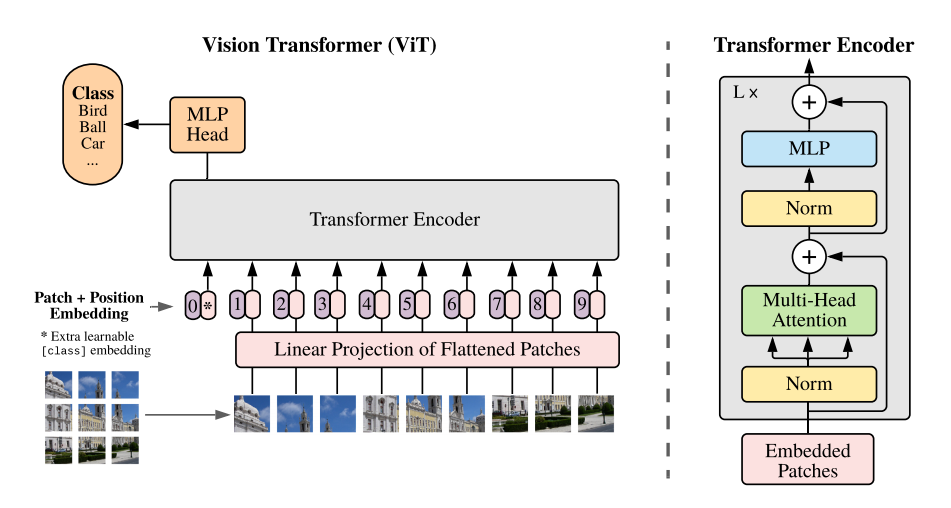
\includegraphics[width=0.8\linewidth]{img_pfe/vit.PNG}
    \caption{Model overview of \textbf{ViT}. We split an image into fixed-size patches, linearly embed each of them, add position embeddings, and feed the resulting sequence of vectors to a standard Transformer encoder. In order to perform classification, we use the standard approach of adding an extra learnable \textit{classification token} to the sequence. The illustration of the Transformer encoder was inspired by \parencite{attention_is_all_you_need}. (Adapted from \parencite{vit})}
    \label{fig:vit}
\end{figure}
% \begin{figure}[H]
%     % \centering
%     \begin{minipage}{0.7\textwidth}
        
%     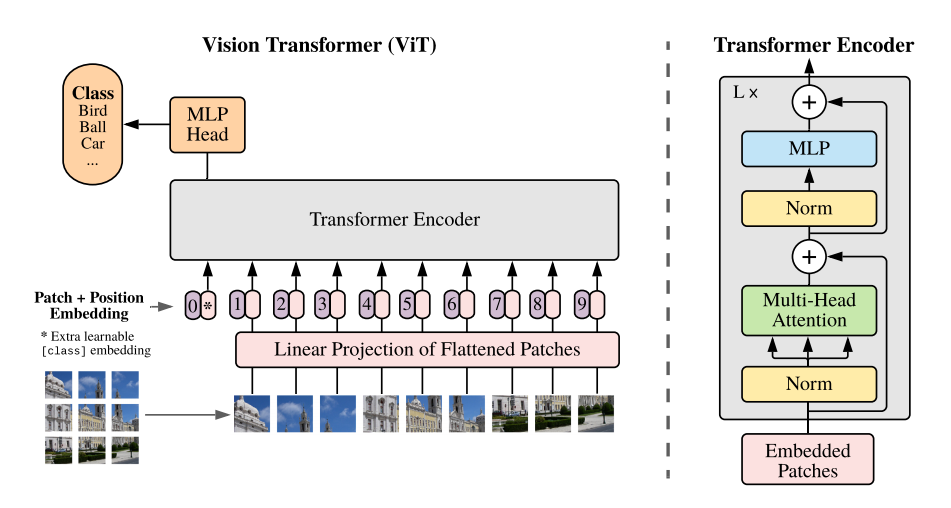
\includegraphics[width=\linewidth]{img_pfe/vit.PNG}
%     \end{minipage}
%     \hspace{0.05\textwidth} 
%     \begin{minipage}{0.2\textwidth}
        
%                 \captionof{figure}{Model overview of \textbf{ViT}. We split an image into fixed-size patches, linearly embed each of them, add position embeddings, and feed the resulting sequence of vectors to a standard Transformer encoder. In order to perform classification, we use the standard approach of adding an extra learnable “classification token” to the sequence. The illustration of the Transformer encoder was inspired by \parencite{attention_is_all_you_need}. (Adapted from \parencite{vit})}
%         \label{fig:vit}
%     \end{minipage}
% \end{figure}
\paragraph{Decoder} 
% A lightweight decoder then reconstructs the full image from the encoded tokens.
a decoder then reconstructs the full image from the encoded tokens.
The decoder takes the encoder's output and reintroduces learnable \texttt{[MASK]} tokens as placeholders for missing patches, each with their correct positional embeddings.Unlike the encoder, the decoder is shallow and computationally inexpensive, as its role is not deep representation learning but rather upsampling high-level features back into pixel space.

\paragraph{Reconstruction loss} Finally, the reconstruction loss provides the learning signal. The model predicts pixel values for masked patches, and the loss \textbf{(Mean Squared Error Equation \eqref{eq:mae_loss})} is computed only on these masked regions, not on visible patches. This ensures that the model focuses on inferring missing information, reinforcing meaningful latent representations. 
The loss function for an image $x$ with masked indices $M$ is:
\begin{equation}
    \label{eq:mae_loss}
    L = \frac{1}{|M|} \sum_{i \in M} \left\| x_i - \hat{x}_i \right\|^2
\end{equation}
where $x_i$ is the original pixel vector for the $i$-th patch and $\hat{x}_i$ is the reconstructed vector.

\subsection*{Key Innovations and Rationale Behind MAE’s Design}
The MAE framework introduces several critical innovations that contribute to its efficiency and effectiveness in self-supervised learning.

\paragraph{High masking ratio} First, the high masking ratio (often 75\% or higher) is a deliberate choice to create a sufficiently challenging pretext task. Natural images contain significant spatial redundancy, meaning that with a low masking ratio, a model could exploit local correlations to reconstruct missing patches without truly understanding high-level semantics. By aggressively masking most of the input, MAE forces the model to develop robust, abstract representations that capture object structure and scene composition.

\paragraph{Asymmetric encoder-decoder architecture} Second, the asymmetric encoder-decoder architecture is central to MAE’s computational efficiency. The encoder, which is the most resource-intensive component due to its deep self-attention layers, processes only the small subset of visible tokens. This reduces both memory usage and training time significantly.
% —by a factor of 3x or more compared to processing the full image. 
Meanwhile, the  decoder handles reconstruction, ensuring that the bulk of the learning occurs in the encoder’s high-level feature space rather than in pixel-level prediction.

\paragraph{Selective reconstruction loss} Another key aspect is the selective reconstruction loss, computed exclusively on masked patches. This design ensures that the model does not simply memorize visible patches but instead learns to infer missing content based on contextual understanding. By focusing the loss on masked regions, LI-MAE encourages the model to develop semantically rich representations that generalize well to downstream tasks.

\paragraph{Tokenization and positional embedding} The tokenization and positional embedding strategy also plays a crucial role. By dividing the image into non-overlapping patches and embedding them with positional information, MAE maintains spatial relationships while converting the input into a sequence suitable for Transformer processing. This approach avoids the inefficiencies of convolutional sliding windows while preserving structural awareness.

% In summary, MAE’s success stems from its carefully balanced design: aggressive masking forces meaningful learning, the asymmetric architecture ensures efficiency, and the reconstruction loss sharpens the model’s ability to reason about missing information. These principles collectively enable MAE to learn powerful visual representations in a scalable, self-supervised manner.

% The MAE architecture and methodology can be broken down into the following key components:

% \begin{description}
%     \item[Input Patching and Masking] The input (e.g., an image) is first divided into a sequence of non-overlapping patches. A large portion of these patches, often as high as 75\%, are randomly removed or ``masked.'' This high masking ratio is crucial, as it makes the reconstruction task non-trivial and prevents the model from simply extrapolating from adjacent patches, forcing it to learn a more holistic understanding of the data.
    
%     \item[Asymmetric Encoder-Decoder Architecture] MAE employs an asymmetric design to process this masked data efficiently.
%     \begin{itemize}
%         \item \textbf{The Encoder:} A high-capacity encoder, typically a Vision Transformer (ViT)\parencite{vit}, operates only on the small subset of visible, unmasked patches. By not processing the masked portions, the computational load during training is significantly reduced (e.g., by 3x or more).
%         \item \textbf{The Decoder:} A separate, lightweight decoder is tasked with the reconstruction. Its input consists of the latent representation of the visible patches (from the encoder) combined with a series of shared, learned ``mask tokens'' that serve as placeholders for the missing patches.
%     \end{itemize}
    
%     \item[Reconstruction Task] The lightweight decoder processes this full sequence of encoded patches and mask tokens to predict the pixel values for only the masked portions of the original input. The model is trained by minimizing a reconstruction loss, such as Mean Squared Error (MSE), between its predictions and the ground-truth values of the masked patches.
% \end{description}

% By learning to predict the missing content from a limited context, the encoder is forced to develop a semantically rich latent representation without requiring any explicit labels, making it a powerful foundation for downstream tasks.
% \section{Architectural Framework}

\section{Architectural Framework}
Our approach is designed as a methodological enhancement to the existing ${MA}^2E$ architecture \parencite{ma2e}. While we do not alter the core network components (the agent's backbone network and the ${MA}^2E$'s Transformer-based auto-encoder), we introduce a novel information flow during the training phase that fundamentally changes how the system learns. This section details the architectural components and the integration of our learning-guided masking mechanism.

The overall framework, as depicted conceptually in  the original ${MA}^2E$  paper \parencite{ma2e}, is composed of two primary parts for each agent:
\begin{description}
    \item[Individual Agent Network (Backbone)] Each agent $i$ possesses its own individual network, which serves as the backbone for the chosen MARL algorithm (e.g., QMIX\parencite{QMIX}(As discussed in Section~\ref{subsec:ctde}  Chapter~\ref{chap:sota}  )). This network, typically a recurrent model like a GRU, is responsible for processing the agent's local action-observation history $h_i$ to produce a hidden state. During the training of our framework, this network also outputs the essential learning signals (such as the Temporal Difference error) that are required to evaluate the agent's performance.
    
    % \item[MA2E Module (Inference Engine)] A shared Transformer-based masked auto-encoder (For more details see Section~\ref{section:mae_original} ) is used by the agents , its role is to take agent trajectories as input and reconstruct them from a masked version. The goal of this module is learning to generate a latent representation that contains global context inferred from partial information.
  \item[$LI-{MA}^2E$  Module ]  Is an inference engine designed to be integrated into existing MARL frameworks \parencite{ma2e}. Its architecture, illustrated in Figure \ref{fig:ma2e_architecture}, is a Transformer-based auto-encoder specifically adapted for multi-agent trajectory data. This section provides a detailed breakdown of each layer in the $LI-{MA}^2E$  pipeline.



% \paragraph{Input Trajectories Layer}
% The foundational data unit for MA2E is not a single state or observation, but a batch of multi-agent trajectories, denoted as $\tau_{t-T+1:t}^{1:n}$. This input, which represents the observation-action histories for all $n$ agents over a time window of length $T$, is structured from the replay buffer into the required sequence format. The reason for using trajectories is that this sequential data contains the essential temporal context required for the model to infer the complex behaviors, intents, and correlations between agents over time.
\begin{itemize}
    \item \textbf{Input Trajectories Layer} The foundational data unit for ${MA}E$ is not a single state but a batch of multi-agent trajectories, $\tau_{t-T+1:t}^{1:n}$, representing the observation-action histories for all $n$ agents over a time window of length $T$. Using full trajectories is crucial because this sequential data contains the essential temporal context required for the model to infer the complex behaviors and intents of other agents.
    \item \textbf{Masking Layer} This layer receives the full sequence of agent trajectories and applies the core masking strategy. As shown in the diagram by the red  \texttt{[X]} markers, the trajectories of a randomly selected subset of $k$ agents are entirely masked out, producing a corrupted sequence where some agents' data is visible and some is hidden. This agent-level masking is a critical design choice tailored to MARL. Unlike masking random patches in an image, masking entire agent trajectories forces the model to solve a more challenging and relevant problem: inferring the complete state and behavior of one agent based on the behavior of others. This directly encourages the model to learn the complex inter-agent dynamics necessary for effective coordination.
    % \item \textbf{Positional Encoding Layer} To provide the necessary sequential context to the permutation-invariant Transformer, this layer adds learnable positional vectors to each token after an initial embedding projection. In MA2E, this is particularly important because the input has two dimensions of order: time and agent ID. Therefore, the positional encoding must capture both, allowing the model to distinguish between, for example, \textit{agent 1 at time t} and \textit{agent 2 at time t}. The paper's\parencite{ma2e} ablation studies confirm that using encodings that consider both agent and time dimensions yields significantly better performance.
    \item \textbf{Positional Encoding Layer}  To provide sequential context to the permutation-invariant Transformer, this layer adds learnable positional vectors to each token after   an initial embedding projection. Since the input has two dimensions of order \textit{time} and \textit{agent ID} the encoding must capture both to distinguish between different agents at different times, for example, \textit{agent 1 at time t} and \textit{agent 2 at time t}. Ablation studies confirm this dual-dimensional encoding is critical for performance \parencite{ma2e}.
    % , enriching the tokens with the structural information needed for the model to succeed.
    \item \textbf{Transformer Encoder Block} Following an asymmetric design for efficiency, a powerful encoder processes only the small, visible subset of unmasked agent trajectories. By applying stacked Multi-Head Attention layers to this sparse input, it learns the complex relationships between agents while using a fraction of the computational resources. Its output is a sequence of latent vectors representing a deep, context-aware encoding of the visible data.
    \item  \textbf{Transformer Decoder Block} The lightweight decoder (shallower and narrower) receives a full sequence of tokens, which is constructed by combining the latent vectors for the visible trajectories (from the encoder) and learnable \texttt{[MASK]} tokens as placeholders for the agents whose trajectories were masked out. Its purpose is not to learn a deep semantic representation, but to perform the final reconstruction task by using the context from the encoded visible tokens to predict the features of the masked tokens. Its output is a full sequence of reconstructed trajectory vectors, $\tilde{\tau}_{t-T+1:t}^{1:n}$.
    \item \textbf{Reconstructed Trajectories (Output Layer)} A final linear projection layer takes the output vectors from the decoder and maps them back to the original dimension of the trajectory data ($o_t^i, u_t^i$). This produces the final reconstructed trajectories for all agents. This output is then compared against the original ground-truth trajectories using a \textbf{Mean Squared Error  loss } function, which in turn generates the gradients that drive the entire learning process.

    
\end{itemize}
% \paragraph{Input Trajectories Layer} The foundational data unit for MA2E is not a single state but a batch of multi-agent trajectories, $\tau_{t-T+1:t}^{1:n}$, representing the observation-action histories for all $n$ agents over a time window of length $T$. Using full trajectories is crucial because this sequential data contains the essential temporal context required for the model to infer the complex behaviors and intents of other agents.
% \paragraph{Masking Layer}
% This layer receives the full sequence of agent trajectories and applies the core masking strategy. As shown in the diagram by the red 'X' markers, the trajectories of a randomly selected subset of $k$ agents are entirely masked out, producing a corrupted sequence where some agents' data is visible and some is hidden. This agent-level masking is a critical design choice tailored to MARL. Unlike masking random patches in an image, masking entire agent trajectories forces the model to solve a more challenging and relevant problem: inferring the complete state and behavior of one agent based on the behavior of others. This directly encourages the model to learn the complex inter-agent dynamics necessary for effective coordination.

% \paragraph{Positional Encoding Layer}
% To provide the necessary sequential context to the permutation-invariant Transformer, this layer adds learnable positional vectors to each token after an initial embedding projection. In MA2E, this is particularly important because the input has two dimensions of order: time and agent ID. Therefore, the positional encoding must capture both, allowing the model to distinguish between, for example, ``agent 1 at time t'' and ``agent 2 at time t''. The paper's ablation studies confirm that using encodings that consider both agent and time dimensions yields significantly better performance, enriching the tokens with the structural information needed for the model to succeed.

% \paragraph{Transformer Encoder Block}
% Following the asymmetric design of the original MAE, a powerful encoder, composed of stacked Multi-Head Attention (MHA) and feed-forward layers, processes only the sequence of tokens corresponding to the visible (unmasked) agent trajectories. The MHA mechanism allows each visible trajectory token to attend to every other visible trajectory token, learning the complex relationships between the agents whose information is available. The rationale for this design is efficiency; by operating on only a small subset of the total data, the most computationally intensive part of the model runs significantly faster and uses less memory, making the entire training process more tractable. The output is a sequence of latent vectors representing a deep, context-aware encoding of the visible trajectories.



 % Its purpose is to use the encoded context from the visible trajectories to efficiently reconstruct the features of the masked ones, outputting a complete sequence of trajectory vectors.

    \begin{figure}[H]
    \centering
      
    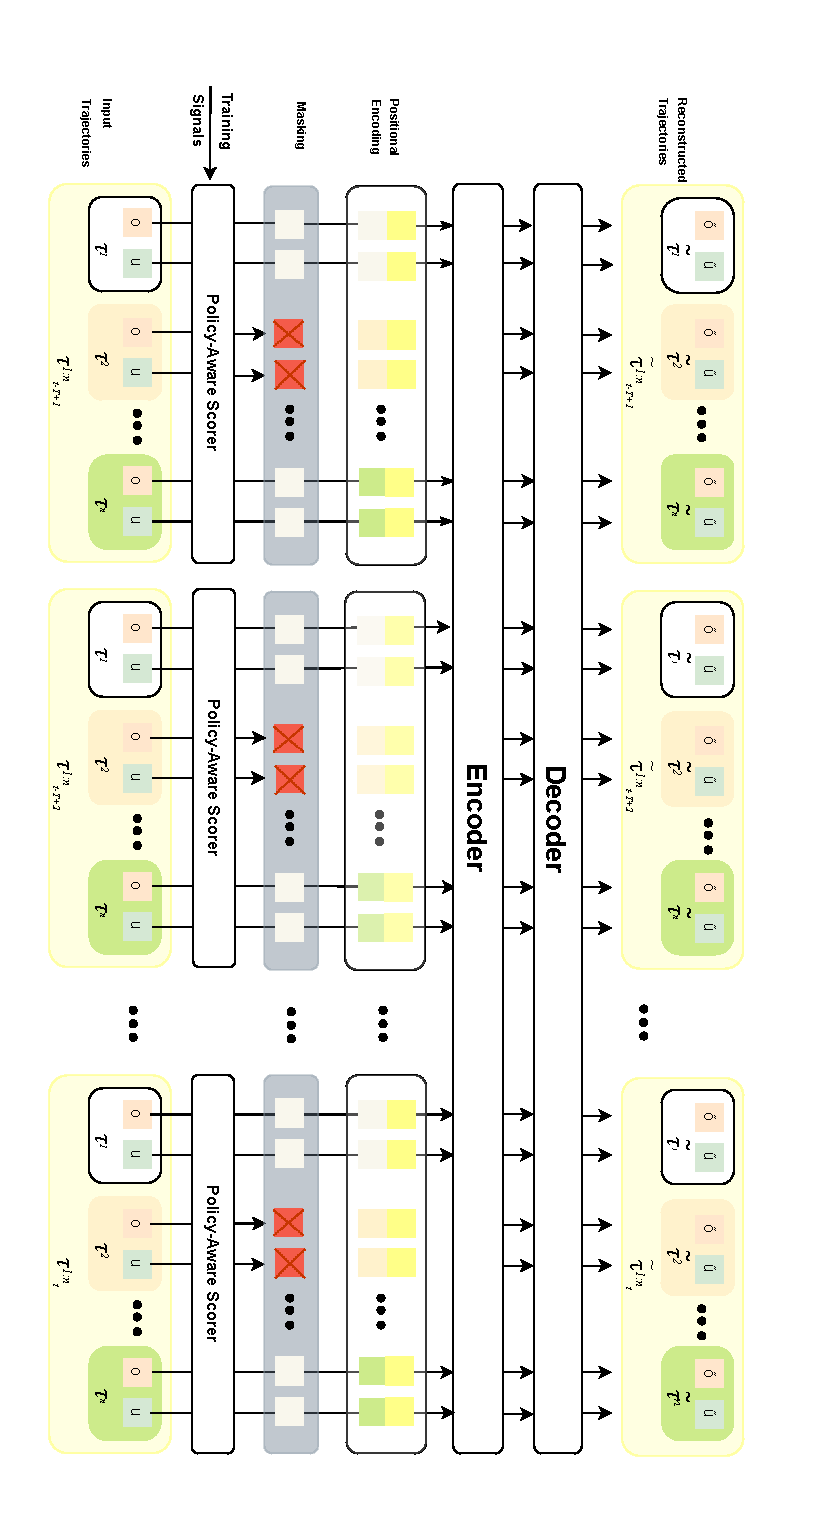
\includegraphics[angle=90, width=0.99\linewidth]{img_pfe/li-mae_this.pdf}
  \caption{The architecture of our proposed \textbf{Learning-Informed Masking ($LI-{MA}^2E$)} framework. Building upon the baseline ${MA}^2E$ , our approach introduces a Policy-Aware Scorer module. During the fine-tuning phase, this module receives training signals (e.g., TD-errors) from the main MARL algorithm and uses them to identify \textit{poorly performing agents}. It then generates a \textit{control signal} that guides the Masking Layer to prioritize masking these specific agents,  forcing the  $LI-{MA}^2E$ module to focus its representational power on reconstructing the trajectories of the most uncertain or poorly performing agents, ensuring the self-supervised task remains Harmonious with the primary reinforcement learning objective.}
    \label{fig:ma2e_architecture}
\end{figure}

\end{description}
% \begin{figure}[htbp]
% \centering

% \caption{The architecture of MA²E. During centralized training, MA²E identifies poor learning agents from all agents' trajectories $\tau_1^1, \tau_1^2, \ldots, \tau_1^k$ and learns to help them improve. The positional encoding is applied considering both the time and the agent information. During decentralized execution, trajectories of poor learning agents are improved while good agents maintain their performance.}
% \label{fig:ma2e_architecture}
% \end{figure}

% \begin{figure}[H]
%     % \centering
%     \begin{minipage}{0.7\textwidth}
        
%     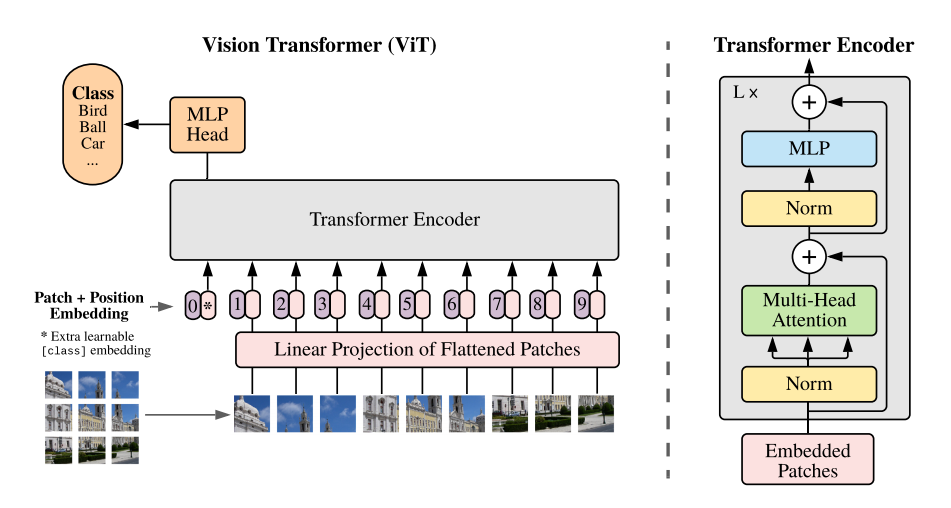
\includegraphics[width=\linewidth]{img_pfe/vit.PNG}
%     \end{minipage}
%     \hspace{0.05\textwidth} 
%     \begin{minipage}{0.2\textwidth}
        
%                 \captionof{figure}{Model overview of \textbf{ViT}. We split an image into fixed-size patches, linearly embed each of them, add position embeddings, and feed the resulting sequence of vectors to a standard Transformer encoder. In order to perform classification, we use the standard approach of adding an extra learnable “classification token” to the sequence. The illustration of the Transformer encoder was inspired by \parencite{attention_is_all_you_need}. (Adapted from \parencite{vit})}
%         \label{fig:vit}
%     \end{minipage}
% \end{figure}

\section{Methodology}
The core of our contribution is a redesigned training methodology that establishes a complementary relationship between the reinforcement learning objective and the self-supervised representation learning task.
% This section provides a detailed, step-by-step explanation of this protocol, following the structure of the original MA2E framework \parencite{kang2025ma2e} upon which it builds.

\subsection{Masking Strategy}
Our framework utilizes a distinct masking strategy for each of its two training phases.
\begin{description}
    \item[During Pre-training (Random Masking)] In the initial phase, we employ the baseline random agent-level masking. The goal is to learn a generalized world model from data collected by a random policy. A subset of $k$ agents is chosen uniformly at random, and their entire observation-action trajectories are masked.
    % This policy-agnostic approach is ideal for this stage as it forces the model to learn general representations without any task-specific bias.
    
    
    \item[During Fine-tuning (Learning-Informed Masking )]  During the main policy training, we replace random masking with  Learning-Informed Masking. Instead of random selection, we identify the \textit{poorly learning} agents within a training batch by using the \textbf{Temporal Difference (TD) error} from the backbone MARL algorithm as a direct performance metric. Agents associated with higher TD-errors are assigned a higher score for being masked. This makes the $LI-{MA}^2E$ focus its representational power on the most uncertain and challenging aspects of the cooperative task.
\end{description}

% \subsection{Core Architecture}
% % The MA2E module itself is a Transformer-based auto-encoder, as illustrated in Figure~\ref{fig:ma2e_architecture}. Following an embedding layer, the input trajectories are processed by a masking layer and a positional encoding layer. This encoding is critical as it must capture the two dimensions of order in the data: the time step and the agent ID. The architecture is asymmetric, with a deep encoder that processes only the visible trajectories and a lightweight decoder that reconstructs the full set from the encoder's output and learnable \texttt{[MASK]} tokens. The encoder and decoder are both built from standard Transformer blocks using Multi-Head Attention (MHA) and feedforward networks.

\subsection{Integration with the Backbone Agent}
The $LI-{MA}^2E$ module is integrated into each agent's individual network to augment its local perception with inferred global context.
\begin{description}
    \item[Parallel Processing] An agent's local history is fed into both its backbone network (e.g., a GRU) and the shared $LI-{MA}^2E$ module.
    \item[Information Fusion via Self-Attention] The reconstructed trajectories from the $LI-{MA}^2E$, $\tilde{\tau}_{1:n}$, are passed to a self-attention mechanism. This layer allows the agent to learn a context-aware summary of the global state by weighing the importance of its teammates' inferred situations relative to its own. The agent's own reconstructed trajectory $\tilde{\tau}_i$ acts as the query, while the others act as keys and values.
    \item[Aggregation] The output of the self-attention layer is then aggregated (e.g., via concatenation) with the hidden state from the agent's backbone network. This fused vector, combining private knowledge with relevant global context, is passed to an aggregation network that produces the final \textit{Q-value} or \textit{policy}.
\end{description}

\subsection{The Training Process:}
The training process is carefully divided into two distinct stages to ensure stability and effectiveness.
\begin{description}
    \item[Stage 1: ${LI-{MA}^2E}$ Pre-training] Before policy learning, the ${LI-{MA}^2E}$ module is trained in isolation on data from a random policy, using the random masking strategy. This is crucial for stability, as it ensures the ${LI-{MA}^2E}$ is already a competent inference engine before the policy begins to rely on it. The module is trained to minimize the Mean Squared Error (MSE) reconstruction loss until it falls below a predefined threshold:
    \begin{equation}
        \label{eq:ma2e_loss}
        L_{\text{LI-${MA}^2E$}} = \frac{1}{nT} \sum_{t=1}^{T} \sum_{i=1}^{n} \left( \tau_t^i - \tilde{\tau}_t^i \right)^2
    \end{equation}
    
    \item[Stage 2: Policy Training and  Fine-tuning] After pre-training, the main MARL training begins. The agent's policy is updated for a set number of steps using the chosen algorithm (e.g., QMIX). This process generates the TD-errors that our Masking  layer  uses to create its  policy-aware mask. The LI-${MA}^2E$  module is then periodically fine-tuned using the same MSE loss, but on data corrupted by this new adaptive mask. This periodic schedule balances stability and adaptability, allowing the policy to learn from a consistent world model while still enabling that model to improve over time based on the agent's learning progress.
\end{description}
% \subsection{Integration with Policy-Aware Masking}
% The novelty of our approach lies in the synergistic integration of these two components. Instead of the MA2E module operating with a random, policy-agnostic masking strategy, its masking process is directly informed by the learning progress of the backbone MARL algorithm. This creates a feedback loop where the reinforcement learning task guides the self-supervised representation learning task.

% The architectural components and data flow are as follows:
% \begin{description}
%     \item[Backbone Individual Network] This is the primary policy or value network for each agent (e.g., a DRQN).
%     \begin{description}
%         \item[What it does:] It processes the agent's local action-observation history to produce a hidden state encoding the agent's private belief.
%         \item[Why we use it:] It serves as the foundation for the agent's decision-making and, crucially for our method, it is the source of the training signals (like TD-error) that quantify the agent's learning progress.
%     \end{description}
    
%     \item[Adaptive Curriculum Masking (ACM) Module] This is the core of our novel contribution.
%     \begin{description}
%         \item[What it does:] This module takes the learning signals from the backbone network as input. It then computes a ``poorly learning'' score for each agent and generates a mask where agents with higher scores are more likely to be masked.
%         \item[Why we use it:] It replaces the policy-agnostic random masking with an intelligent, policy-aware curriculum. This ensures that the MA2E's representational power is focused on the agents that need the most assistance.
%     \end{description}
    
%     \item[MA2E Inference Engine] The standard MA2E auto-encoder.
%     \begin{description}
%         \item[What it does:] The encoder takes the visible (unmasked) agent trajectories as input and produces a latent representation. The decoder then attempts to reconstruct the masked trajectories.
%         \item[Why we use it:] It is the engine that performs the self-supervised learning, generating a rich representation that contains inferred global information.
%     \end{description}
    
%     \item[Aggregation Network] A final network layer that fuses information.
%     \begin{description}
%         \item[What it does:] It takes as input both the hidden state from the agent's backbone network and the latent representation from the MA2E encoder. It then aggregates these two sources of information.
%         \item[Why we use it:] It allows the agent to combine its private knowledge with the inferred global context, creating a final, comprehensive representation for decision-making.
%     \end{description}
% \end{description}

% The training process, which will be detailed in the subsequent sections, is briefly composed of a pre-training phase with random masking to establish a general world model, followed by a fine-tuning phase where our policy-aware ACM module is employed to create a targeted learning curriculum.
\subsection{The Critical Role of Pre-training in Representation Learning}
A core methodological choice in our framework is the use of a two-phases during  training : a self-supervised pre-training phase followed by a task-specific fine-tuning phase. This \textit{pre-train, fine-tune} paradigm is not an arbitrary design choice, but a foundational principle in modern machine learning that is essential for achieving stable and high-performing models. This section justifies the necessity of the pre-training stage .

The primary reason for using pre-training is to decouple initial representation learning from downstream task learning, thereby preventing unstable learning dynamics. Attempting to train a MARL policy and  MAE concurrently from scratch creates a vicious cycle : the MARL policy, initially random, generates poor-quality data, which prevents the world model from learning a useful representation. In turn, this inaccurate world model provides noisy and misleading information back to the policy, destabilizing its learning process. Pre-training breaks this cycle by first developing a competent and generalized world model, which then provides a robust foundation for the policy to learn from.

The power of this paradigm was first demonstrated conclusively in the field of \ac{NLP} with the introduction of \ac{BERT} \parencite{bert_pretraining_deep_bidirectional_transformers_language_understanding}. The \ac{BERT} paper revolutionized NLP by showing that a deep Transformer model could be pre-trained on a simple, self-supervised objective : predicting randomly masked words from a massive unlabeled text corpus. By learning to solve this \textit{Masked Language Model} task, the model was forced to develop a deep, contextual understanding of language. The key finding was that this pre-trained model could then be adapted to a wide variety of downstream tasks (e.g., question answering, sentiment analysis) by adding just one task-specific layer and fine-tuning the entire network Figure~\ref{fig:bert_architecture}. This established that a  pre-trained representation could serve as a powerful and transferable foundation, solidifying the \textit{pre-train, fine-tune}  strategy as a dominant approach in the field.
\begin{figure}[H]
    \centering
   
        
    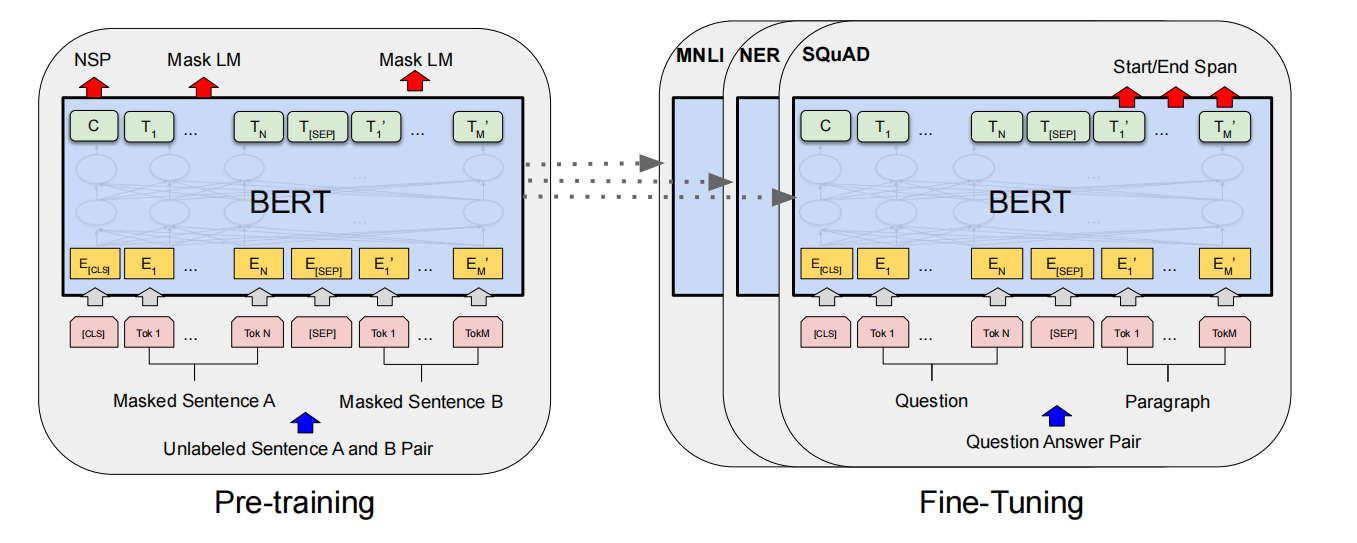
\includegraphics[width= 0.9\linewidth]{img_pfe/bert.png}
 
  
                \caption{Overall pre-training and fine-tuning procedures for BERT. Apart from output layers, the same architectures are used in both pre-training and fine-tuning. The same pre-trained model parameters are used to initialize models for different down-stream tasks. During fine-tuning, all parameters are fine-tuned. \texttt{[CLS]} is a special
symbol added in front of every input example, and \texttt{[SEP]} is a special separator token (e.g. separating questions/answers).(Adapted from \parencite{bert_pretraining_deep_bidirectional_transformers_language_understanding})}
        \label{fig:bert_architecture}
\end{figure}
Building directly on this success, the \textbf{BEiT (Bidirectional Encoder representation from Image Transformers)} \parencite{beit_bert_pretraining_image_transformers} paper successfully translated this paradigm to the domain of computer vision . The authors explicitly state their motivation as adapting the BERT-style pre-training for image data. To overcome the challenge that images lack a natural vocabulary like text, BEiT introduced a two-stage process: first, an image is \textit{tokenized} into a sequence of discrete visual tokens using a separate auto-encoder. Then, during pre-training, the model is given a version of the image where some patches are masked, and its objective is to predict the correct visual tokens for those masked patches. BEiT's success demonstrated that the core principle of learning a representation through a masked reconstruction task is not limited to language but is a powerful and generalizable strategy. This work reinforces the idea that establishing a robust foundational model through a self-supervised pre-training phase is a standard and necessary step before proceeding to task-specific fine-tuning.


More recently, this pre-training philosophy has been directly and successfully applied to the domain of \textit{sequential decision-making and reinforcement learning}. The \textbf{Masked Decision Prediction (MaskDP)} framework illustrated in Figure ~\ref{fig:MaskDP} \parencite{mae_scalable_generalizable_decision_making}
explicitly uses a masked auto-encoder, pre-trained on state-action trajectories, to create a scalable and generalizable agent . The central idea is that by pre-training the model to reconstruct randomly masked states and actions from a trajectory, it learns a rich understanding of the environment's dynamics. The authors \parencite{mae_scalable_generalizable_decision_making} demonstrate that this single, pre-trained model can then be applied to various downstream tasks, such as \textit{goal-reaching} or \textit{offline RL} , often in a \textit{zero-shot manner}. This powerfully reinforces the core idea that a pre-training phase on a self-supervised reconstruction task is a highly effective strategy for learning a versatile and transferable world model that can be efficiently adapted for specific decision-making problems.
\begin{figure}[H]
    \centering
   
        
    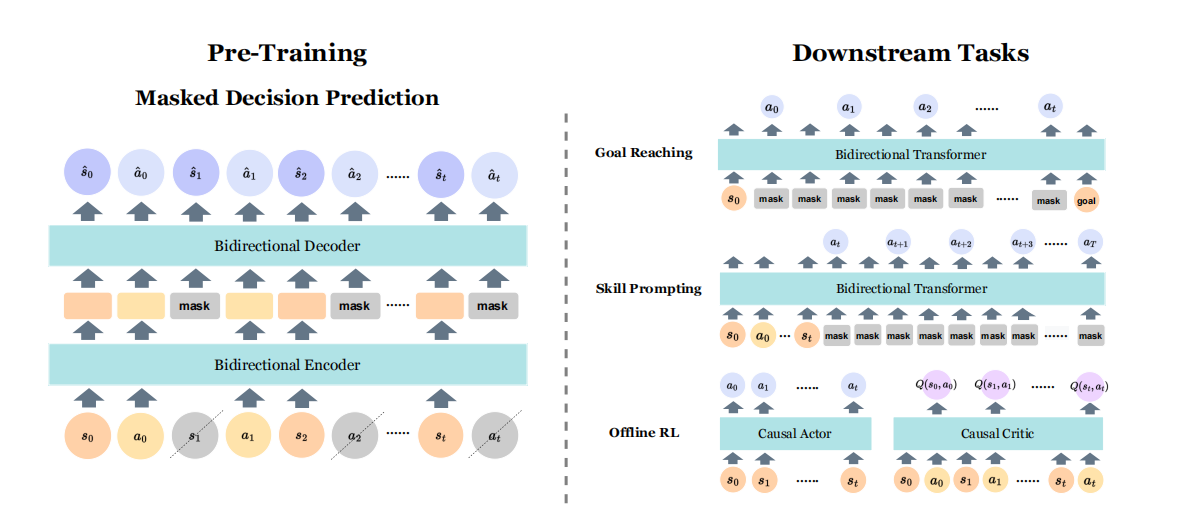
\includegraphics[width= 0.9\linewidth]{img_pfe/mae_Scalable_and_Generalizable_Decision_Making.PNG}
 
  
                \caption{Illustration of MaskDP. During \textit{pretraining} stage, we perform the masked token prediction task. And after pretraining, the model can be deployed to various downstream tasks using different mask patterns.(Adapted from \parencite{mae_scalable_generalizable_decision_making})}
        \label{fig:MaskDP}
\end{figure}
In recent years, this pre-training philosophy has been directly and successfully applied to the domain of sequential decision-making and reinforcement learning. The work on \textbf{Masked World Models (MWM) for visual control} \parencite{masked_world_models_visual_control} explicitly argues for \textit{decoupling visual representation learning} from \textit{dynamics learning }. The authors \parencite{masked_world_models_visual_control}  contend that training a single model end-to-end for both objectives creates a detrimental trade-off that prevents the model from capturing the \textit{fine-grained visual details} necessary for complex robotic control . Their solution is a two-stage process where an auto-encoder is first trained on a masked reconstruction task to learn a rich visual representation. Only after this representation is learned is a separate latent dynamics model trained on top of these powerful, pre-trained features . This explicit separation prevents the dynamics learning objective from interfering with the visual learning objective, providing strong evidence that a pre-trained visual model offers a superior foundation for subsequent RL tasks .


Similarly, the \textbf{Masked Trajectory Models (MTM)  framework} \parencite{masked_trajectory_models_prediction_representation_control} showcases the extreme 	flexibility that a pre-trained model can offer . MTM pre-trains a single, general-purpose model on a unified task: reconstructing randomly incomplete state-action trajectories. The key insight is that a single model, pre-trained in this way, can be used for a multitude of downstream tasks without any retraining. By simply changing the masking pattern at inference time, the model can function as an offline RL agent, a forward dynamics model, or an inverse dynamics model. This powerfully illustrates that a robust, pre-trained representation of environment dynamics is not only transferable but can also be highly versatile, accelerating and in some cases even replacing the need for specialized downstream models. Together, these works provide strong support  that a two-stage protocol, beginning with a self-supervised pre-training phase to learn a robust world model, is a critical component for achieving stable, efficient, and high-performing results in complex decision-making domains.

\section*{Conclusion}

This chapter detailed our primary contribution :\textbf{the Learning-Informed Masking Framework ($LI-{MA}^2E$)} . We began by deconstructing the principles of the Masked Auto-Encoder, establishing it as a powerful tool for self-supervised representation learning. We then presented our novel framework, which introduces a \textbf{Policy-Aware Scorer} module that integrates directly with the backbone MARL algorithm. The core of our methodology is a two-phase training process: an initial pre-training stage with random masking to build a general world model, followed by a fine-tuning stage where our \textbf{Learning-Informed Masking} uses signals like the TD-error to focus the MAE's representational power on the most uncertain agents. By creating this direct link between the reinforcement learning objective and the self-supervised reconstruction task, our framework ensures the two remain aligned, fostering a more efficient and effective learning curriculum. Having formally defined this new methodology, the next chapter will provide a comprehensive empirical validation of its performance.

Having formally defined this new methodology, a critical design question remains:\textbf{What is the most effective metric for identifying a 'poorly performing' agent in a way that best serves the representation learning task?}  The next chapter will address this directly, beginning with a methodical investigation into several candidate scoring functions before presenting a comprehensive empirical validation of the final, optimized framework.